\subsection{Division of Tasks}
WRITTEN BY DENNIS 
Whenever new tasks were brought up at group meetings they were initially divided into parts and subcomponents that could be iteratively delegated to each member of the group. For instance, the requirements analysis document sections were marked as tasks which could either be worked on individually or in groups. The group members have chosen tasks independent from time consumption and scope as one does not know this until they have worked with the given task.\\\\ Each member was to work on a given task single-handed although if a distributed task was exceedingly great, it was either divided even further or was assigned with additional members. However, the group does analyze in some degree if a given task had a tremendous impact  for the whole project and was thus regarded as a task that demanded the whole group's focus. By example, when working on the Design Goals in the system design document the whole group was required to work on this section before they could proceed with the document. \\\\The distribution of work/tasks for each part of the project can be seen on figur \ref{fig:rad}, figur \ref{fig:sdd} and figur \ref{fig:codeskeleton}. Notice how each task is divided into sections that are delegated to each member. Each member had some main tasks that they were responsible for (which can be seen on the high percentage). However, one may also notice that other members do have a smaller percentage on some given tasks. This is because the given task was either too great, difficult or because the other member was simply done with their own task and was, therefore, placing their resources into other tasks.


% RAD TIME TABLE 
\begin{figure}[H]
	\centering
	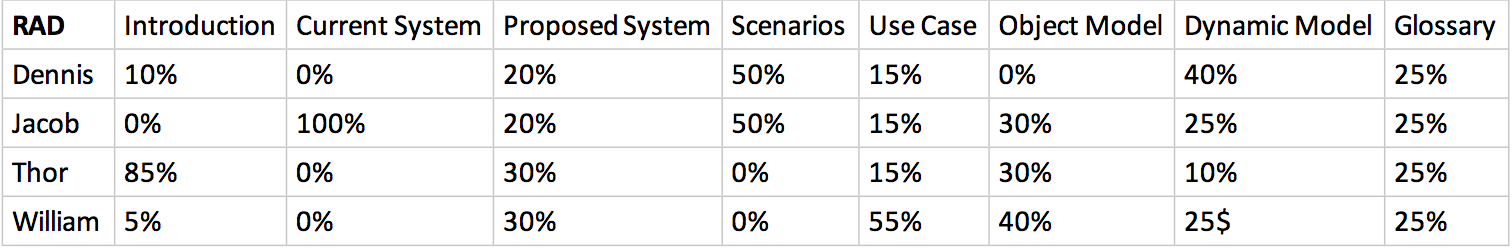
\includegraphics[width=150mm]{radtimetable}
	\caption{RAD Work Distribution}
	\label{fig:rad}
\end{figure}

% SDD TIME TABLE 
\begin{figure}[H]
	\centering
	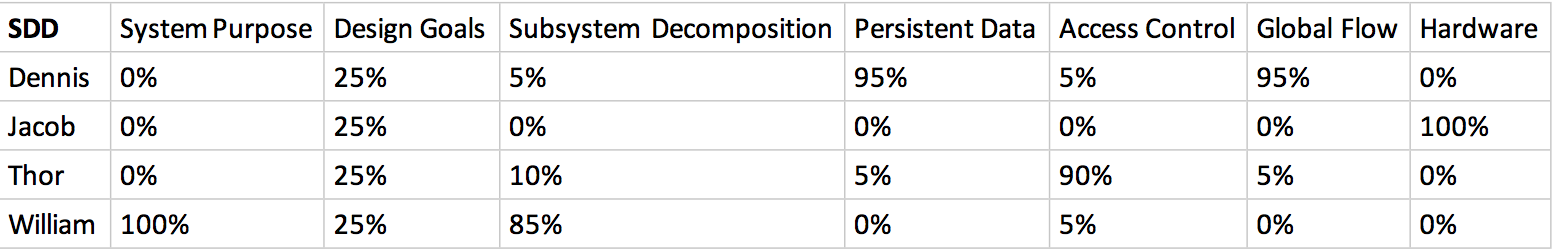
\includegraphics[width=150mm]{sddtimetable}
	\caption{SDD Work Distribution}
	\label{fig:sdd}
\end{figure}

% Code Skeleton TIME TABLE 
\begin{figure}[H]
	\centering
	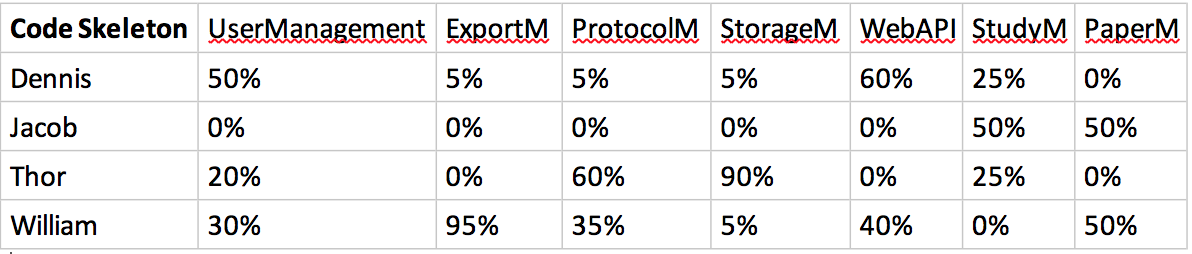
\includegraphics[width=150mm]{image/skeletontimetable}
	\caption{Code Skeleton Work Distribution}
	\label{fig:codeskeleton} % To use write \ref{fig:codeskeleton}
\end{figure}
